\documentclass[../relazione.tex]{subfiles}
\graphicspath{{\subfix{../images/}}}
\begin{document}
\section{Prima implementazione funzionante}
Per la prima implementazione si è usato un array che contenesse il peso dei singoli task e una matrice di adiacenza per rappresentare gli archi e cioè le dipendenze tra i nodi. 

L'algoritmo è diviso in tre fasi, ricerca degli entrypoint, 
calcolo delle metriche e ordinamento dei task. Per tutte le fasi sono stati implementati dei kernel OpenCL in modo da poter essere eseguiti su GPU.

\subsection{Fase 1 - Ricerca degli entrypoint}
Si scandisce il grafo in cerca dei nodi che non hanno nessun genitore, e cioè dei task che non hanno nessuna dipendenza e di cui si può calcolare immediatamente la metrica.

\begin{lstlisting}[language=C++, caption={Find entrypoints kernel},captionpos=b]
kernel void entry_discover(const int n_nodes, global edge_t* restrict edges, volatile global int* n_entries, global int* entries)
{
	int current_node_index = get_global_id(0);
	if (current_node_index >= n_nodes) return;

	for (int j = 0; j < n_nodes; j++) {
		int matrixToArrayIndex = matrix_to_array_indexes(j, current_node_index, n_nodes);
		if (edges[matrixToArrayIndex] > 0) {
			return;
		}
	}
	entries[current_node_index] = 1;
}
\end{lstlisting}

\subsection{Fase 2 - Calcolo delle metriche}
Si aggiungono gli entrypoint ad una coda e per ogni elemento della coda si calcola la metrica. 
La metrica di un task è una coppia in cui il primo elemento è dato dal peso del nodo che indica la mole di lavoro e quindi di tempo che il task impiega prima di terminare, mentre il secondo elemento è il livello, cioè la profondità massima a cui si trova nel grafo (se quindi un task $t_1$ ha due genitori $\{p_1, p_2\}$, il suo livello sarà dato da $max\_level(p_1, p_2) + 1$).
Inoltre per ogni nodo in coda, dopo averne calcolato la metrica, si aggiungono in coda i suoi task dipendenti e la procedura si ripete fino a quando la coda non si svuota.


\begin{lstlisting}[language=C++, caption={Compute metrics kernel},captionpos=b]
kernel void compute_metrics(global int * restrict nodes, global int *queue_, global int *next_queue_, const int n_nodes, global edge_t* restrict edges, volatile global int2 *metriche /*<RANK,LIVELLO>*/)
{
	int current_node_index = get_global_id(0);
	[...] //omissis of various security checks
	for(int j = 0; j<n_nodes; j++){
		int parent = j;
		int matrixToArrayIndex = matrix_to_array_indexes(parent, current_node_index, n_nodes);
		int edge_weight = edges[matrixToArrayIndex]; 
		if(edge_weight > 0){
			int weight_with_this_parent = edge_weight + metriche[parent].x + nodes[current_node_index];
			int level_with_this_parent = metriche[parent].y+1;
			int2 metrics_with_this_parent = (int2)(weight_with_this_parent, level_with_this_parent);
			if(gt(metrics_with_this_parent, metriche[current_node_index]))
				metriche[current_node_index] = metrics_with_this_parent;
		}

		int child = j;
		matrixToArrayIndex = matrix_to_array_indexes(current_node_index, child, n_nodes);
		int adiacent = edges[matrixToArrayIndex];
		if(adiacent > 0){
			atomic_inc(&next_queue_[child]);
		}
	}
}
\end{lstlisting}

Questo kernel tuttavia deve essere eseguito dall'host più di una volta, in particolare verrà invocato fin quando la \textit{next\_queue} risultante non sarà identica a quella del ciclo precedente, cosa che indicherà che il kernel non ha fatto cambiamenti nell'ultimo ciclo e ha quindi terminato.

\subsection{Fase 3 - Ordinamento dei task}
Una volta calcolate le metriche di tutti i task, l'insieme dei task viene ordinato nel seguente modo:
\begin{enumerate}
    \item Si ordinano in base al livello in modo crescente
    \item I task di pari livello vengono ordinati in base al proprio peso in modo decrescente.
\end{enumerate}

\begin{lstlisting}[language=C++, caption={MergeSort kernel for metrics couple array, source: \url{https://github.com/Gram21/GPUSorting}},captionpos=b]
__kernel void merge_sort(const __global int2* inArray, __global int2* outArray, const uint stride, const uint size)
{
	const uint baseIndex = get_global_id(0) * stride;
	if ((baseIndex + stride) > size) return;
	const char dir = 1;
	uint middle = baseIndex + (stride >> 1);
	uint left = baseIndex;
	uint right = middle;
	bool selectLeft;

	for (uint i = baseIndex; i < (baseIndex + stride); i++) {
		selectLeft = (left < middle && (right == (baseIndex + stride) || lte(inArray[left], inArray[right]))) == dir;

		outArray[i] = (selectLeft) ? inArray[left] : inArray[right];

		left += selectLeft;
		right += 1 - selectLeft;
	}
}
\end{lstlisting}

\subsection{Considerazioni}
Dato $n$ numero di nodi, la complessità di questa prima implementazione è $O(n^2)$ per la ricerca degli entrypoint, $O(n^2)$ per il calcolo delle metriche e $O(n\ log\ n)$ per l'ordinamento.

In definitiva, l'algoritmo ha complessità $O(n^2)$ e, come vedremo in dettaglio fra poco, il maggior peso in termini di runtime si riscontra nella Fase 2, per cui ci focalizzeremo maggiormente su quest'ultima fase d'ora in poi.

\subsection{Variazioni}
Per provare ad abbassare i tempi di runtime troppo alti dei kernel con questa implementazione si sono provati vari approcci:
\begin{itemize}
    \item Per prima cosa abbiamo provato a lavorare con una matrice di adiacenza trasposta sperando di migliorare i tempi di accesso della GPU alla memoria, con scarso successo.
    \item In seguito abbiamo provato ad ottimizzare il codice in modo che venisse eseguito il più possibile in GPU perché fino a questo momento l'host prendeva il controllo ad ogni ciclo rimandando in input al kernel la coda che il kernel stesso aveva popolato. Anche in questo caso i risultati sperati non sono sopraggiunti.
    \item Come ultimo tentativo si è deciso di vettorizzare l'algoritmo nella speranza che facendo fare più lavoro ai singoli work item i tempi di runtime diminuissero, nella realtà però si è ottenuto il risultato opposto.
\end{itemize}    
Riportiamo di seguito i risultati dei test eseguiti con l'algoritmo originale e 
le sue variazioni su un dataset di 4096 task su GPU NVIDIA GTX 1650 per 15 esecuzioni di cui successivamente è stata calcolata la media dei tempi di runtime.

\begin{figure}[H]
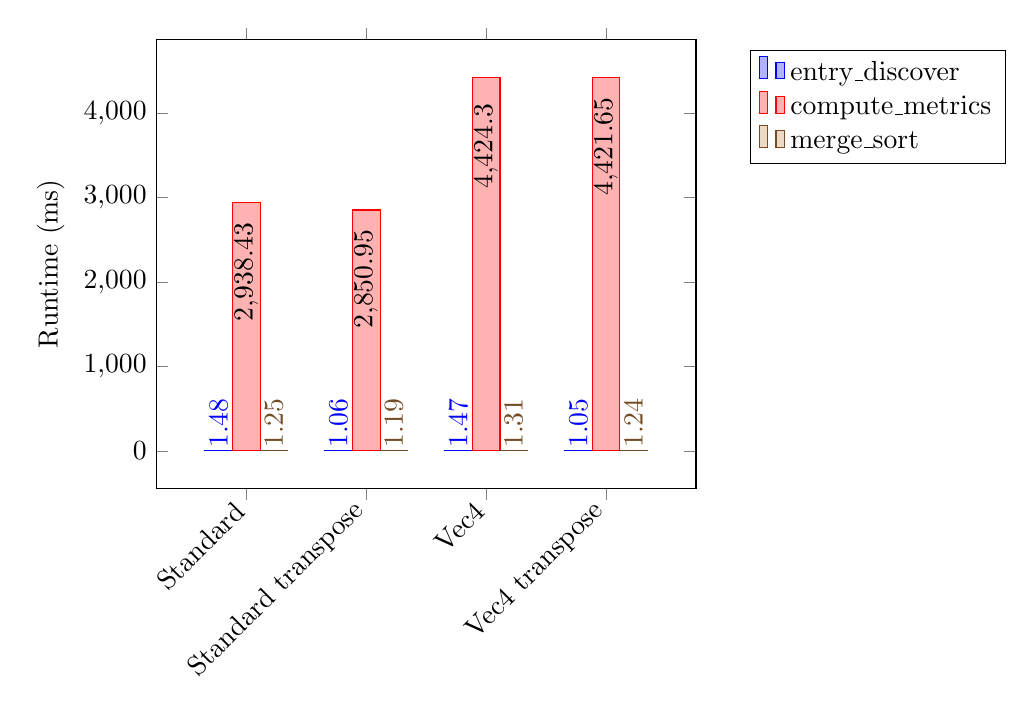
\begin{tikzpicture}
\begin{axis}[
symbolic x coords={
Standard,
Standard transpose,
Vec4,
Vec4 transpose},
x tick label style={rotate=45,anchor=east},
nodes near coords,
every node near coord/.append style={rotate=90, anchor=center},
ylabel=Runtime (ms),
legend style={at={(1.1, 0.85)}, anchor=west},
ybar=0pt,
legend cell align={left},
enlarge x limits=0.25,
]
\addplot+[every node near coord/.append style={yshift=10pt, xshift=20pt}] coordinates { %entries discover
(Standard, 1.48) (Standard transpose, 1.06)
(Vec4, 1.47) (Vec4 transpose, 1.05)
};
\addplot+[every node near coord/.append style={xshift=-25pt, color=black}] coordinates { %compute metrics
(Standard, 2938.43) (Standard transpose, 2850.95)
(Vec4, 4424.30) (Vec4 transpose, 4421.65)
};
\addplot+[every node near coord/.append style={yshift=-10pt, xshift=0pt}] coordinates { %mergesort
(Standard, 1.25) (Standard transpose, 1.19)
(Vec4, 1.31) (Vec4 transpose, 1.24)
};
\legend{entry\_discover, compute\_metrics, merge\_sort}
\end{axis}
\end{tikzpicture}
\caption{Tempi di runtime della prima implementazione}
\end{figure}
\end{document}